\begin{table*}
	\centering
	\begin{tabular}{| c | p{0.25\textwidth}|c |c |c || c |c |c |}
	
	
 	    \multicolumn{2}{c}{} & \multicolumn{3}{c}{Web Traffic} 		  & \multicolumn{3}{c}{File Transfer} \\
 	     \cline{3-8}	
             \multicolumn{2}{c|}{} & CPU 			& Memory (Mb) 		& Throughput (Mbps)	& CPU 		& Memory (Mb)		& Throughput (Mbps) \\\hline   
Settings 1 & client connected to the gateway with ip forwarding &   3.6\% 		& 693 		& 11.461		& 2.7\%		& 708 Mb		& 11.455 \\\hline
Settings 2 & client connected via squid proxy hosted on the gateway   &   52\%        & 692 		& 11.455		& 47\%		& 703 Mb		& 11.450 \\\hline
Settings 3 & client connected to SvNF proxy hosted on the gateway with no rule deployed &   66\%		& 680 		& 11.404		& 54\%		& 707 Mb		& 11.449 \\\hline
Settings 4 & client connected to SvNF proxy hosted on the gateway with 10,000 rules deployed   &   69\%        & 690 		& 11.430		& 56\%		& 704 Mb		& 11.444 \\\hline
	
	            
	\end{tabular}
	\caption{
	OSGi HTTP proxy performance comparison
	\label{tab:perf-comparison}
	}
	
\end{table*}

Section~\ref{sec:migrating} described the role of SvNF deployed on the HG and the server-side infrastructure composed of various vNFs: Streamers vNFs deployed in regional PoPs, Caching and Transcoding Orchestrator and Transcoding vNFs deployed in regular data-centers. 

As our proposal aims at showing how software deployed in a modular HG can play a role in a vNF architecture, our first focus for the evaluation is devoted to assessing HG side performance, CPU and memory footprint.
Next, to evaluate the benefits of the overall SvNF+vNF system in above-cited use case, we made extensive simulations with hypothesis conforming exactly to the french network of Service Provider "Orange".

\subsection{SvNF Evaluation }\label{Testbed}

We deployed the SvNF OSGi bundle in the Apache Karaf OSGi runtime on an \textit{PC Engines APU/1C} gateway\footnote{http://www.pcengines.ch/apu1c.htm} running Debian Jessie. 
The APU/1C gateway is built upon a low-power AMD Bobcat x86 microarchitecture and 2Gb or RAM, with 3 Gigabit Ethernet channels. Its raw performances are comparable to current Home Gateways models recently launched on the market\footnote{For example, FreeBox mini 4K's Brahma15 ARM7 processor scores 2 cores x \textbf{5.250Dmip} @ 1500 Mhz while APU/1C scores 2 cores x \textbf{2.560 Dmip} @ 1000 Mhz}, this assures the reproducibility of the results. The gateway connects the test operator and a PC-based file server.

%\begin{figure}
%  \begin{center}
%    
\includegraphics[width=0.30\textwidth]{fig/testbed.pdf}
%  \end{center}
%  \caption{ SvNF Performances testbed
%    \label{fig:testbed}
%  }
%\end{figure}	



JMeter\footnote{http://jmeter.apache.org} was used to capture the network metrics of our solution.
While generating HTTP requests, it reports on specific performances metrics. Each experiment consisted of 10 agents continuously downloading target resources on the HTTP file server, 1000 times.

We considered two different validation use-case: Web Traffic and File Transfer. First, the agents had to download a 192 MB video file, then a single HTML page which linked to 171 static resources composed of Javascript files, CSS and images of average size 16 KB.

We evaluated our solution with two different rules settings deployed in the SvNF. In the first one, we did not deploy any rule, assessing only the overhead linked to the application network framework. In the second one, however, we deployed 10.000 rules, causing the SvNF to process both requests and responses wrt those rules thereby assessing its ability to perform pattern matching in a timely manner. Both cases reflect the no operation scenario of our use-case, as  presented in ~section \ref{noop}.

We decided to assess the overhead caused the SvNF by comparing it to the well-known Squid 3 HTTP proxy. To have a better grasp of the amount of resources consumed by the SvNF, we also reported CPU and memory consumption for each settings as well.

From ~Table \ref{tab:perf-comparison}, we can see that the performances in term of throughput is globally the same across all settings, with the maximum deviation from the baseline setting 1 (simple ip forwarding) being less that 0.3\%.
In settings 2-4, we also see that a significant share of CPU power is dedicated to processing the requests for both Squid 3 and the SvNF, with the SvNF consuming up to a 25\% extra CPU time in Settings 4 wrt Settings 1, but with no drop in throughput. This can be explained by the fact that the SvNF runs on top of a JVM, while Squid is a native application with limited overhead wrt a Java application.

As this experiment does not intend to mimic real life Internet usages but to stress the system up its limits.
We conclude that even with the extra CPU involved, our solution does not significantly penalize the End-User, validating the possible deployment of SvNFs on modular Home Gateways.

\subsection{Performance study of Content Distribution} \label{videodelivery}
\begin{table}
	\scalebox{0.8}{
		\begin{tabular}{| l | l | l|}
		\hline
			\textbf{Settings} & \textbf{Scenario A} & \textbf{Scenario B}\\\hline
			CP Bandwidth &2 Gbps&1 Gbps\\\hline
			Regional PoP Bandwidth &0 Gbps&1 Gbps\\\hline
			Regional PoP latency& \multicolumn{2}{l|}{25ms} \\\hline
			CP latency& \multicolumn{2}{l|}{50ms} \\\hline
			Video Distribution& \multicolumn{2}{l|}{Normal} \\\hline
			Video Size&\multicolumn{2}{l|}{Pareto with average video size=10Mb}\\\hline
			Requested bitrate &\multicolumn{2}{l|}{320kbps}\\\hline
			\# of gateways &\multicolumn{2}{l|}{ 200}\\\hline
			\# of video (cruising/peak) &\multicolumn{2}{l|}{ 200/100}\\\hline
			Mean time between request (cruising/peak) &\multicolumn{2}{l|}{ 0.1s/0.05s (Poisson))}\\\hline
			SLA Violation criteria &\multicolumn{2}{l|}{ less than 75\% of the target bitrate 10s after the request}\\\hline
			Video Caching&\multicolumn{2}{l|}{after 4 requests}\\\hline
		\end{tabular}
	}
	\caption{Hypothesis used for simulation\label{simu1}}
\end{table}
We simulated the network deployment presented in ~Figure \ref{fig:hld}, with the specifications presented in ~Table \ref{simu1}.

The objective is first to assess the feasibility of having a SvNF+vNF approach and second to highlight its benefits. 
The use case considers the deployment of SvNF in the HG and vNF in the SP's regional PoPs, for video delivery.
Let us thus investigate the potential of such a solution.

Streamed video need good bitrate to avoid re-buffering and improve QoE. That is the reason why we defined an SLA violation as the failure to deliver the proper average bitrate on time to a client. Our goal in this simulation is to reduce the SLA violations over time.

The regional PoP being located near the End-User, its latency is reduced wrt the CP network (backed by CDN), hence a possible higher throughput for HTTP traffic like video streaming.
For our simulation, we included two types of patterns. The first one is composed of video requests emitted regularly by the clients, which generate a cruising phase traffic. The second consists of traffic at \textit{25s} which is characterized by a greater request arrival rate as well as a more concentrated distribution of videos. Consumption peaks usually occur when a viral video is posted, most of the time on the landing page of the Content Provider. Being able to cache this kind of video and to serve it as close as possible to the users is a key indicator of success for the vNF.
\begin{figure}
  \begin{center}
    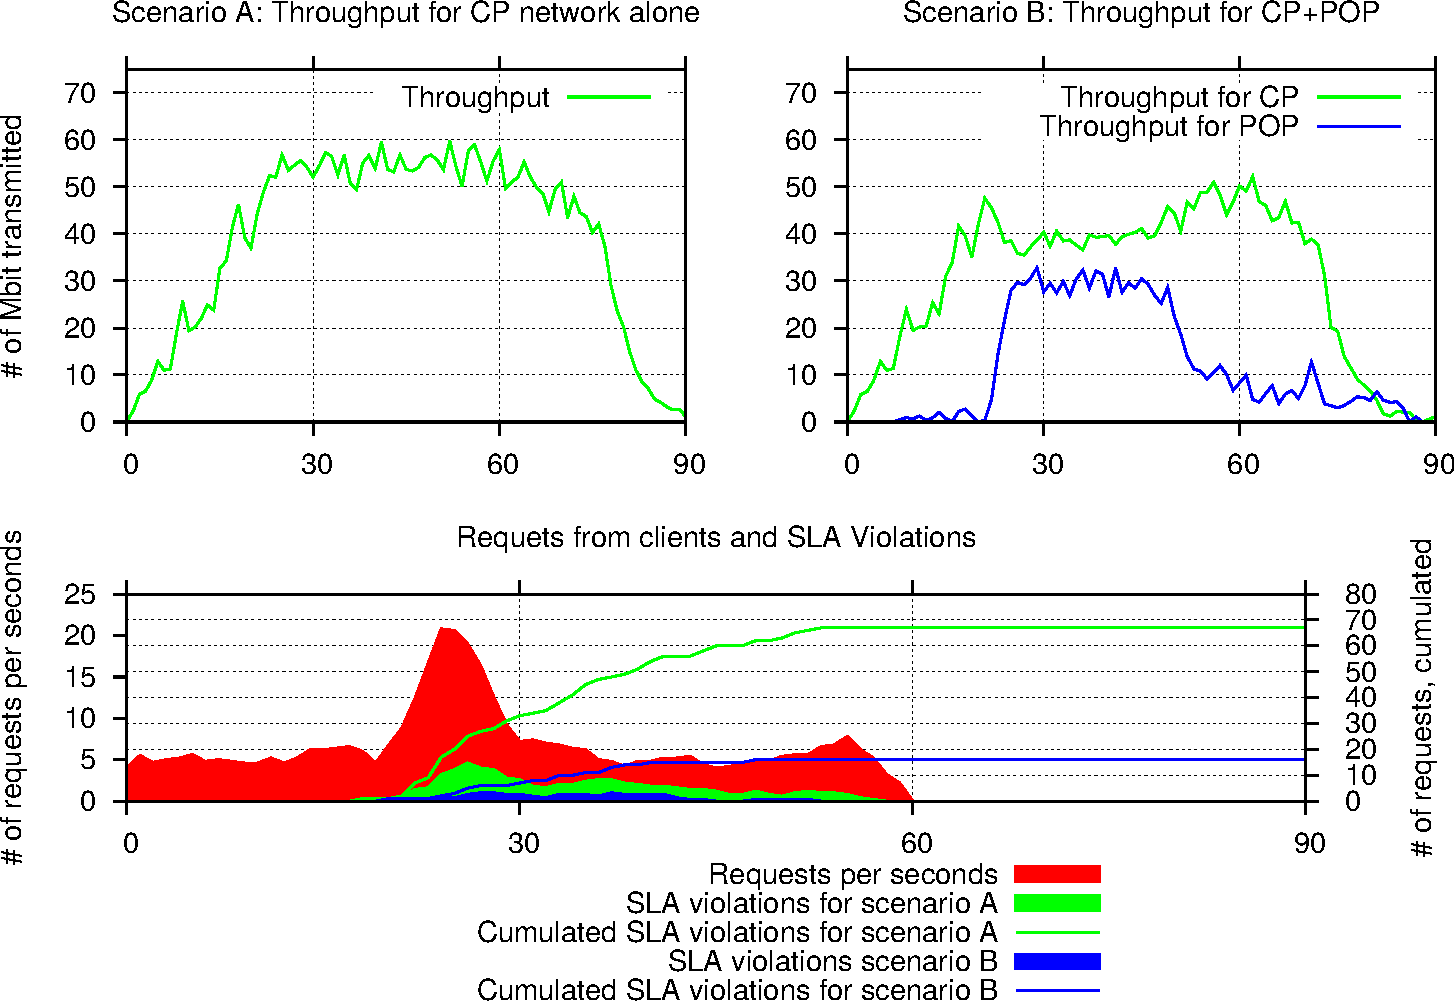
\includegraphics[width=0.45\textwidth]{fig/CP+POP_evaluation.pdf}
  \end{center}
  \caption{ Evaluation of the benefits of the SvNF+vNF system
    \label{fig:cppopeval}
  }
\end{figure}	

Figure~\ref{fig:cppopeval} depicts two scenarios. In (A), we only rely on CP network to deliver the media while in (B) a single regional PoP is added to the solution. 
Note that global bandwidth remains the same, as we took some bandwidth from the CP to allocate it to the regional PoP.
This is also essential for the CP for comparing at the end the solutions in terms of bandwidth cost.

We can see that the cruising phase does not generate any SLA violation and the CP alone is able to handle the traffic load. However, when the peak occurs, SLA violations increase dramatically, causing a lot of requests to be dropped. In scenario B, however, the presence of the regional PoP as an alternative, low latency data source, mitigate the peak effect and reduces up to 70\% of SLA violations to on the overall simulation period.

Having a regional PoP with lower network latency to serve highly redundant requests, benefits to both the user and the content provider. As the former sees an increase in QoE, the latter reduces cost by avoiding the over provisioning of network capabilities. It's important however, to reserve regional PoP bandwidth to serve only highly popular videos, so as to maximize its benefits, while keeping the mean latency low between clients and regional PoPs by spreading PoPs along the territory.

\subsection{Performance study of provisioning decisions} \label{provisionningdecisions}


\begin{figure}
	
 \begin{center}
    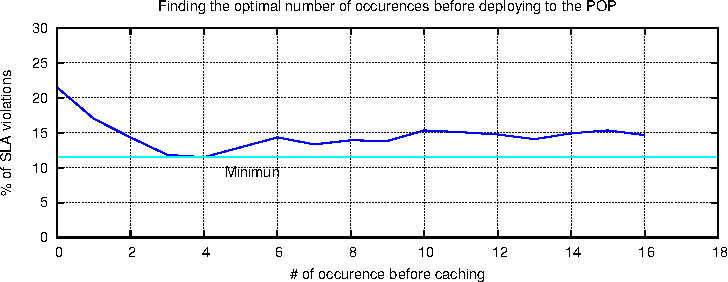
\includegraphics[width=0.45\textwidth]{fig/cachingStrat_evaluation.pdf}
  \end{center}
  \caption{ Caching Strategy Evaluation
    \label{fig:cachingstrateval}
  }
\end{figure}	

Regional PoPs are designed to have great network performances, and need to be distributed through the territory for a reduced price.
In order to mitigate the storage cost, the caching controller takes the decision to provision as few videos as possible to fulfill the SLA. Several factor can influence the decision, like the transcoding time, the vNF booting time, hosting costs and so on.
Taking the decision to provision a video in a specific regional PoP means classifying the video as cachable according to some meta data, like the view count in a certain time window.
In \cite{silvestre_boosting_2015}, the authors proposed a model for predicting the popularity of a video, and estimated that view counts accounted for 82\% of the relative importance. 
We implemented a very simple provisioning policy, based on the number of views for the same resource received in a 10 minutes rolling window. If the number is above the threshold, the video is cached at the regional PoP level and clients can download the video from there.

~Figure \ref{fig:cachingstrateval} shows that for our particular settings, the value that minimize the percentage of SLA violation is 4. This can be explained by the fact that we want to preserve the regional PoP for serving only the most popular videos (which will trigger the most SLA violations) and not clutter it with less popular videos that could be easily served by the CP. However, as the propagation of the caching policy takes time, we want to react promptly and not wait for too many popular videos to hit the CP.

In production, this evaluation should be updated regularly by monitoring the overall traffic and the network conditions and possibly using other video meta data.





